\documentclass{article}
\usepackage{tikz}
\pagestyle{empty}
\begin{document}
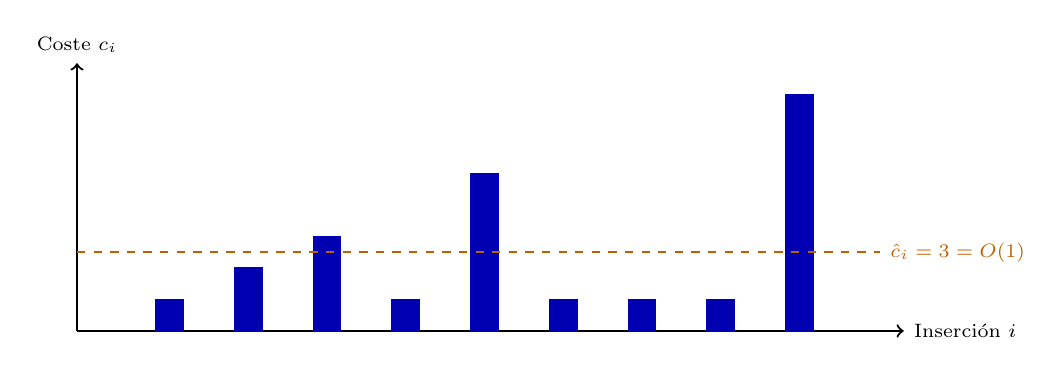
\begin{tikzpicture}

\draw[thick, ->] (0,0) -- (10.5,0) node[right, font=\scriptsize] {Inserción $i$};
\draw[thick, ->] (0,0) -- (0,3.4) node[above, font=\scriptsize] {Coste $c_i$};
\foreach \x/\h in {1/0.4, 2/0.8, 3/1.2, 4/0.4, 5/2.0, 6/0.4, 7/0.4, 8/0.4, 9/3.0} {
    \filldraw[blue!70!black] (\x,0) rectangle (\x+0.35,\h);
}
\draw[dashed, orange!75!black, thick] (0,1.0) -- (10.2,1.0) node[right, font=\scriptsize] {$\hat{c}_i = 3 = O(1)$};

\end{tikzpicture}
\end{document}
